%
% zahlengerade.tex
%
% (c) 2026 Prof Dr Andreas Müller
%
\begin{figure}
\centering
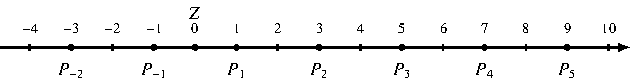
\includegraphics{papers/basel/images/zahlengerade.pdf}
\caption{Grenzübergang: Der Kreis $k_n$ wird zur Zahlengeraden durch $Z = 0$.
Die Punkte $P_k$ liegen bei den ungeraden Zahlen
$\ldots, -3, -1, 1, 3, 5, \ldots$
im Abstand $1, 3, 5, 7, \ldots$ von $Z$.
\label{basel:figure:gerade}}
\end{figure}
